\begin{enumerate}

    \item 
        The upper bound on the number of misclassified instances can be given as $$\sum_{i=1}^{n}\xi_{i}$$
        
    \item 
        $C$ [\ref{fig:3_a}] is the variable that controls the trade-off between the classification accuracy and the margin of the linear separators. In other words, it determines the influence of misclassification on the objective function.
    
        As $C \rightarrow \infty$, the resulting hyperplane would have relatively smaller margin given it is able to better separate the classes.
        
        As $C \rightarrow 0$, the optimizer would choose a relatively smaller margin hyperplane even if that hyperplane misclassifies a few samples. It would act as a regularization effect on the optimization.
    
        \begin{figure*}[!ht]
            \centering
            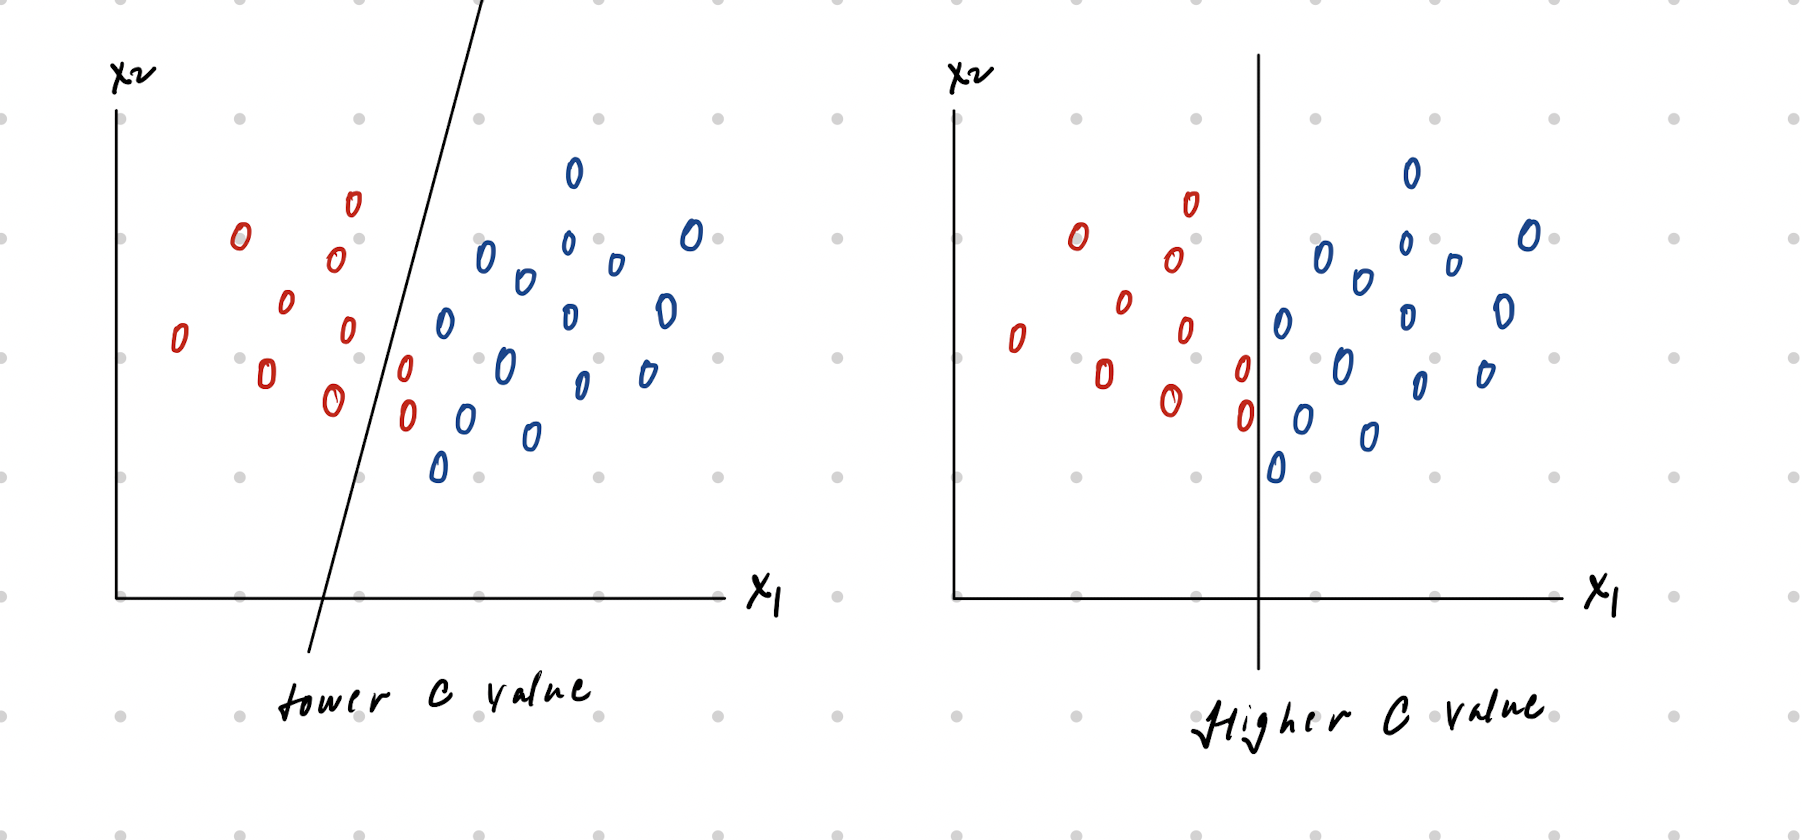
\includegraphics[width=\textwidth]{images/problem_3_a}
            \caption{Influence of $C$}
            \label{fig:3_a}
        \end{figure*}

    \item        
        We can consider the dual primal relationship $$\phi(x_{i})^{T}\phi(x_{j}) = k(x_{i}, x_{j})$$. Now, the estimate for a sample can be given as 
        \begin{align*}
            \hat{y} & = sign(w^{T}\phi(x)) \\
            & = sign(\sum_{i=1}^{n} \alpha_{i}y_{i}\phi(x_{i})^{T}\phi(x)) \\
            & = sign(\sum_{i=1}^{n} \alpha_{i}y_{i}k(x_{i}, x_{j}))
        \end{align*}
        The kernel trick uses $k(x_{i}, x_{j})$ instead of $\phi(x)^{T}\phi(x_{j})$. Therefore, predictions can be made using $k(x_{i}, x_{j})$ instead of using the $\phi(x)$ function.
        
        
\end{enumerate}